\clearpage
\newpage % 开始新的一页
    \thispagestyle{empty} % 移除本页的页眉和页脚[8,9](@ref)
    \newgeometry{margin=0pt} % 临时将本页的页边距全部设置为0[1](@ref)
    \noindent % 防止缩进
    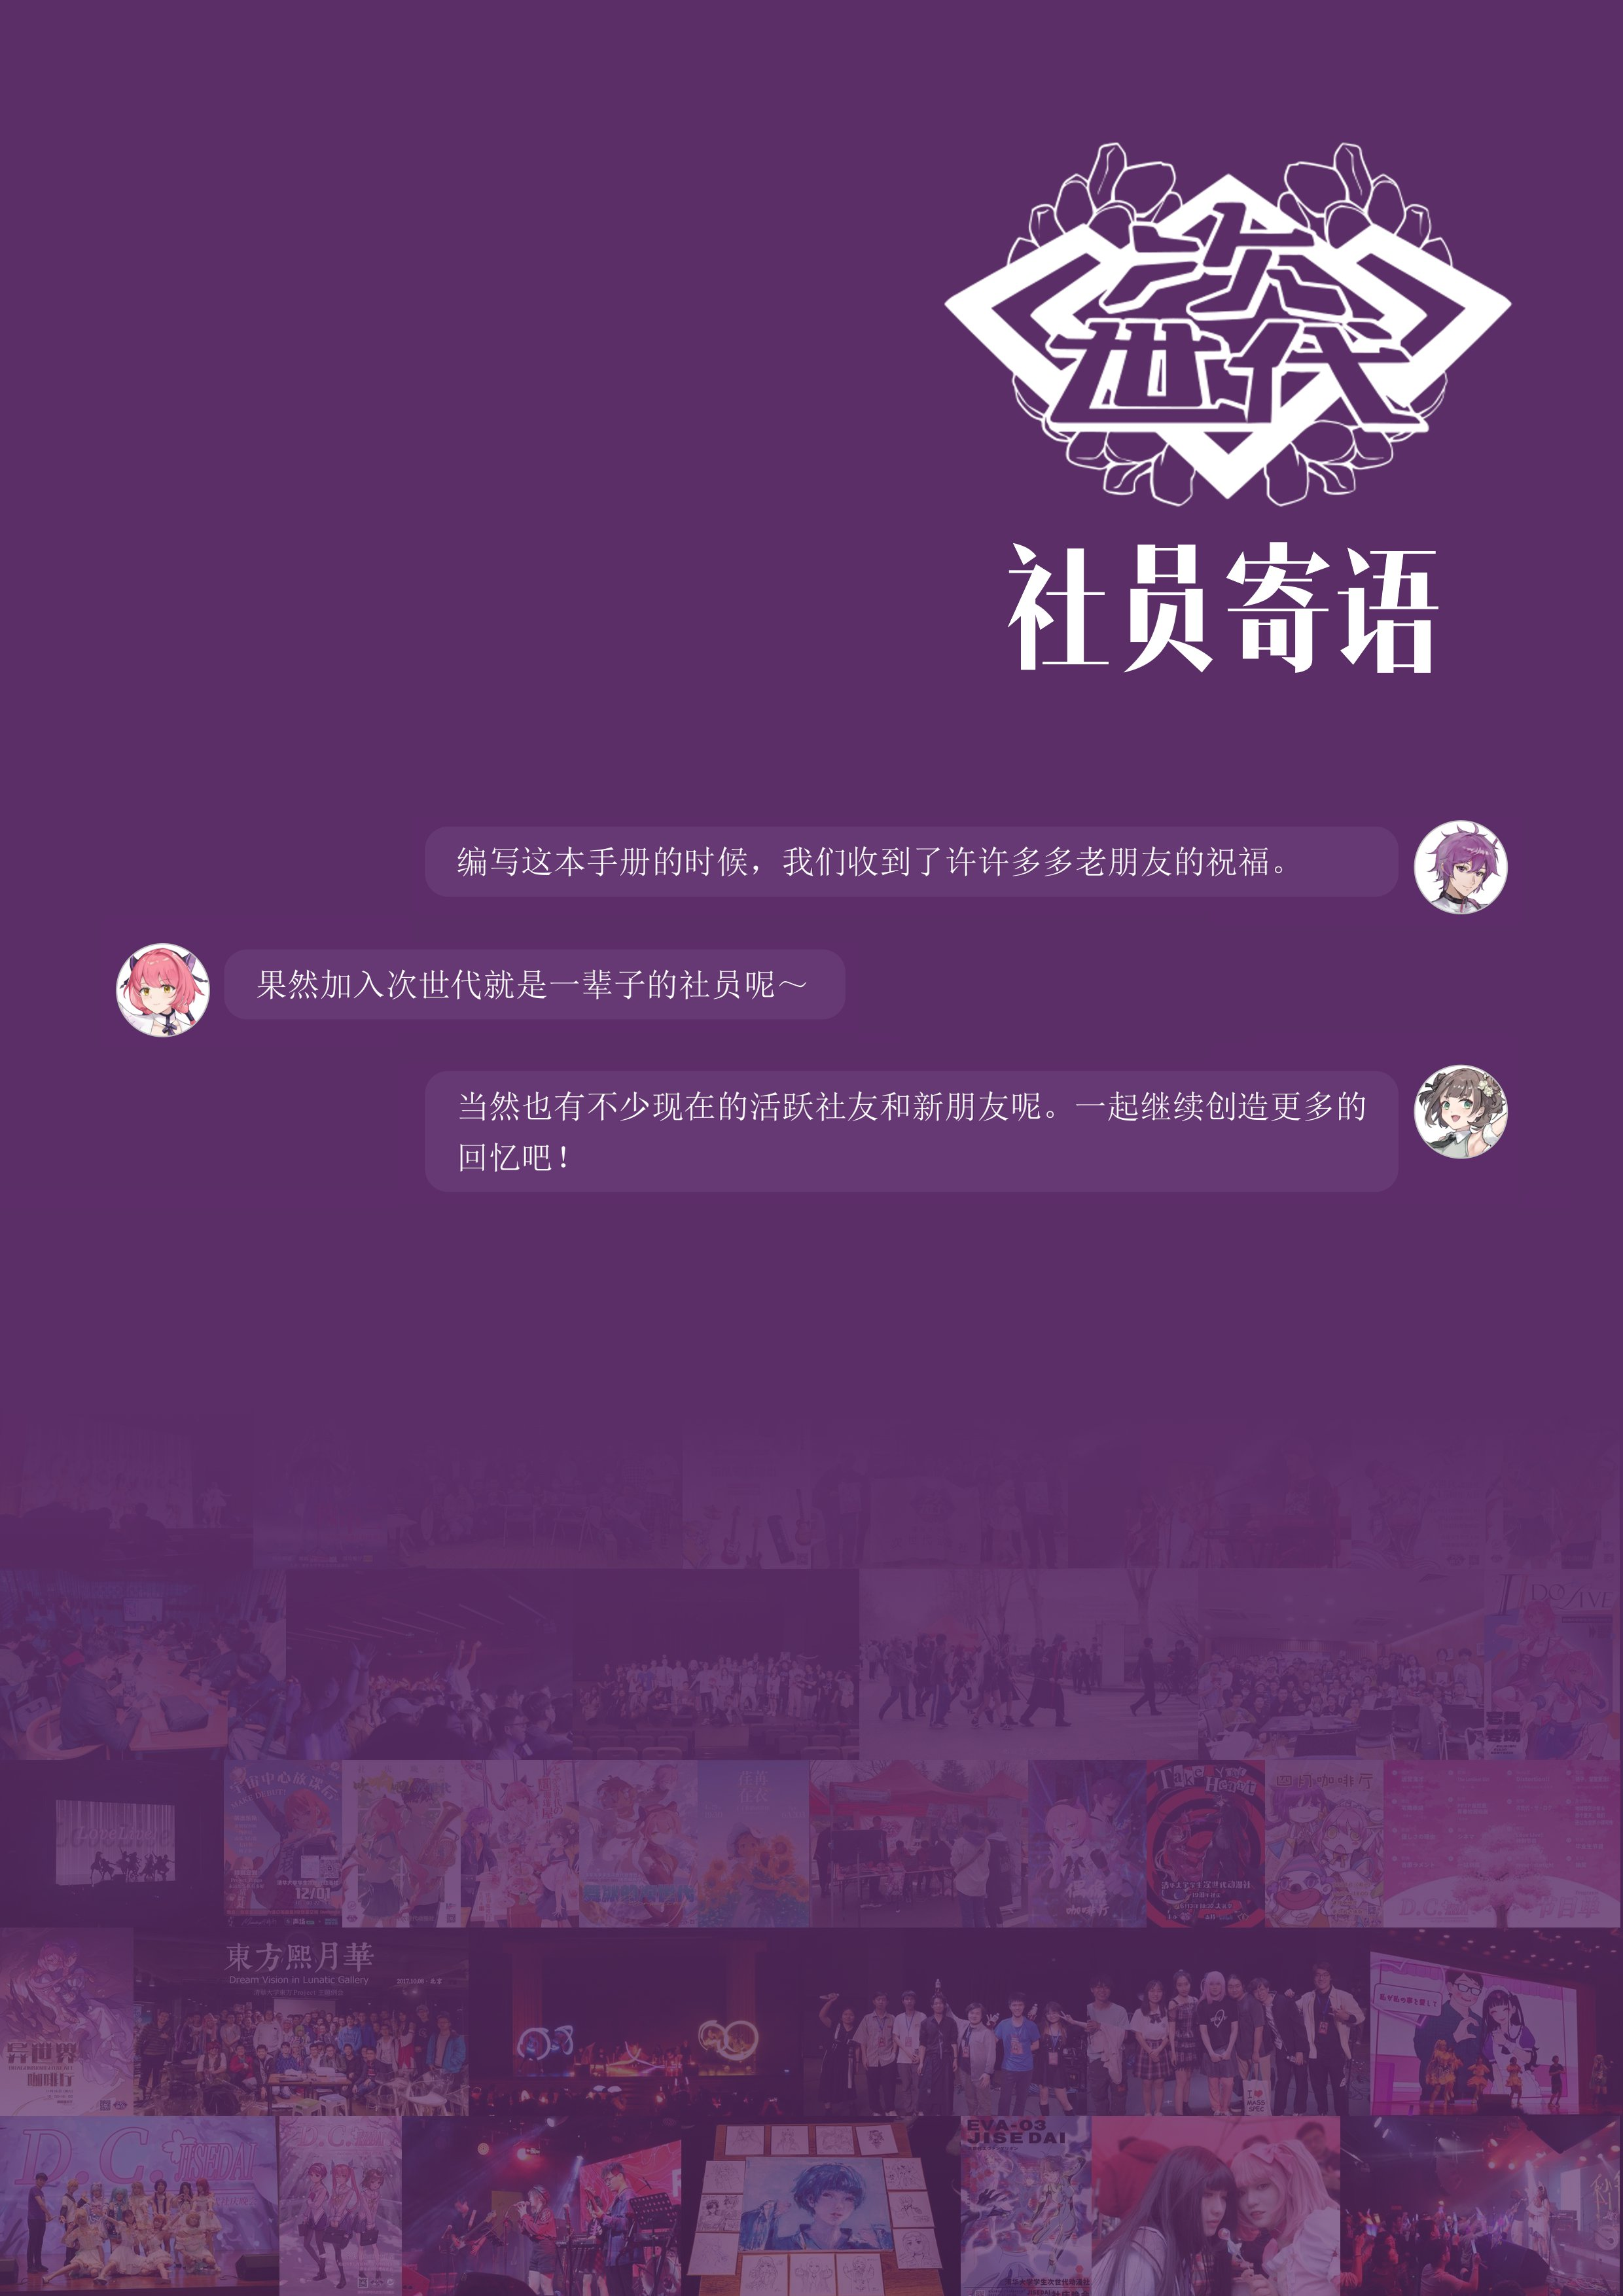
\includegraphics[width=0.9999\paperwidth, height=0.9999\paperheight]{ch5.jpg} % 插入图片,使其尺寸与纸张大小一致并保持宽高比[1](@ref)
    \restoregeometry % 恢复原来的页边距设置
\newpage
\normalsize

\chatbubble[right]{Koyou.jpg}{22-Koyou 深度砖工}{
没有加入你社的话我大学生活估计会少大半乐趣。
}{zi}

\chatbubble[left]{阿茗.jpg}{22-阿茗不吃鱼~~25届副社长、宅舞部部长+组织部重度依赖\emoji{💜}}{%
跳舞很开心!搞cos很开心!拍照很开心!\\办活动很开心!大自习很开心!一起玩很开心!\\
欢迎加入宅舞部一起跳舞(幻想n年后宅舞部什么样子)\\
顺便祝大家早日脱单(抓走组织部长x)
}{default}

\chatbubble[right]{展颜.jpg}{22-展颜 \emoji{🐳}}{
\emoji{💜👍💃👍👏👏🙌👏👏🎉🎉🎉💃💃💃👍👍👍}
}{zi}

\chatbubble[left]{江枫.jpg}{14-江枫~~18届社长}{%
我的本科四年也是在次世代的四年,感觉每天做的事见的人度过的时光都和次世代紧紧相连着。
可以说次世代在某种程度上塑造了我,也深深地影响着离开校园的我。\\
希望次世代的家人们都能在这里获得属于自己丰满的美好的回忆~
}{default}

\chatbubble[right]{雨绫.jpg}{21-雨绫~~虽然喜欢的很多但既然是东方部管理所以大家来搞东方(?}{
次世代仿佛一个坚实的锚点,在每个人不一定一帆风顺的大学生活中,或许平时很难意识到,
事后回想才会发现原来平日的悲欢里都有它的影子。要相信在这个形形色色的人交织而成的团体中,
一定可以寻找到值得你珍视的线哦。
对了,在校期间一定要参与一次社庆吧,把你的热爱告诉所有人,留下独属于自己的痕迹!
}{zi}

\chatbubble[left]{寒月.jpg}{19-寒月}{%
开学的时候从百团大战加入的次世代,这里个个都是人才,说话又好听!找到了很多游戏、动漫同好,水群花了很多时间!
}{default}

\chatbubble[right]{沙包.jpg}{10-沙包}{
好怀念紫荆的麻辣香锅。
}{zi}

\chatbubble[left]{天海兰.jpg}{17-天海兰~~无限想念华子的毕业社畜学长}{%
感谢次世代,尤其是次世代东方部的伙伴们,曾经一起开例会,与全市车万人相聚,一起出发听幻奏盛宴,去玩东方only,这些记忆闪耀了我的大学时光。
}{default}

\chatbubble[left]{梧桐明夜.jpg}{20-梧桐明夜~~绘画部退休部长}{%
\chind 次世代是一个实现梦想的故事。从最早到这里了寻找一起搞彩虹小马的人,到在绘画部学画画,
再到进组织部干活、上台讲相声,我在次世代的每一步都走得出乎意料却充满获得感。
最早的时候,在次世代参加的每一次活动都会有新的悸动。总会产生我想在次世代完成这个,参与那个的期待。
顺着这些期待走去,在快乐的时光中,它们也一个个变成了现实。画了海报、上了社庆、当了部长,
总能看到一个个悸动开花结果。

\chind 曾记得一位社友说过:“次世代不是给人分发任务的地方,而是发现有谁想要做什么,
然后利用社团资源帮他实现想法的地方。”在次世代,只要敢想就能敢做。
在这里你能看到关于动漫和大学社团的所有幻想变成三次元的真实。

\chind 次世代也是一个找到自己价值的地方。丰富多彩的活动背后是每位社友的鼎力支持和倾情付出。只要你愿意成为其中的一部分,
总会有适合你的岗位,让你在社团活动中留下独属于自己的烙印。每次办完大型活动,
我都有一种身处热血番末尾的感觉。看着身为Staff的大家在散场音乐中合影,互道一声辛苦,
收拾自己的东西奔向聚餐。

\chind 你的每个闪光点都是次世代急需的宝藏,哪怕你自己都不曾意识到。
部门拟人的部酱企划本来是我一时兴起自娱自乐的产物,用于表达我入社四年来在各个部门的所见所感。
没想到能得到社友们的厚爱,甚至变成了DV剧搬上社庆。只要献出你独特的爱,在次世代,总会有用你的钥匙才能打开的门锁。

\chind 次世代绘画部是一个家一样的地方。大家在里面各自发画,相互夸夸,一问一答,相约线下。
最近的每次茶绘都能挤满C楼的教室。大家说说笑笑,交换无料,在同一张画布上描绘自己的心迹。绘画部的人都很温柔,
绘画部的空气都很清新。无论你是大触还是新手,都能在这里找到归属。
}{default}

\chatbubble[right]{撒旦.jpg}{18-撒旦~~被迫隐身虾饺传说}{
Helden sterben nicht!祝次世代的大家永远不死~
}{zi}

\chatbubble[left]{TerryWScheler.jpg}{23-TerryWScheler~~加入原神部谢谢喵}{%
希望能像玛拉妮一样每天都很乐观
}{default}

\chatbubble[right]{砂53.jpg}{25-砂$5^3$~~究极百合骑士}{
出勤时受到博士老登感化加入次世代\\
应该是你社为数不多百团前就加入的小登\\
(是的 主播开学第四天就穿着系服出勤了喵)\\
诸君,请玩音游吧!
}{zi}

\chatbubble[left]{四号线.jpg}{21-四号线~~关注星瞳official谢谢}{%
路过的观众,请容我向您介绍一位出色的虚拟偶像-星瞳,关注星瞳喵,关注星瞳谢谢喵。星瞳是 FPS 游戏高手、全民 k 歌黄金段位拥有者、舞者、歌手、小说家、相声演员、画师。
}{default}

\chatbubble[right]{无解.jpg}{20-无解~~加入东方部/轻小说部/日语学习部谢谢喵}{
在你社留下了很多回忆,也认识了很多朋友,是和大家一起玩的回忆支撑我走过了在校的时光。
次世代这种纯粹地在“玩”而没有什么内卷和功利心的地方是非常珍贵的,
欢迎大家在这里走错(啊不)迈出自己的大学第一步
}{zi}

\chatbubble[left]{疾风.jpg}{20-疾风}{%
其实一开始没打算加学校动漫社这种现充俱乐部(刻板印象)的,
不过被社友朋友介绍的三人成部吸引于是还是速速入社摇人成立了IDOLiSH7部哈哈哈。
因为自由宽松的建部和入部制度,次世代有着多种多样的兴趣部门且可以同时参加,
得益于此,即便是我这样的社恐老废宅,只需要一点勇气,也能在次世代体验了第一次参本、
参与社庆舞台灯光工作、组织JSD48×IDOLiSH7舞蹈节目、参演舞台剧(虽然因为疫情变DV剧了)和配音节目、
和社友出去唱K……感谢次世代,给予了我很宝贵的回忆。
}{default}

\chatbubble[right]{恒斌.jpg}{18-恒斌~~(曾)ktn单推人}{
加入次世代,走错人生第一步(bushi\\
然后加入galgame部,走错人生第二步(bushi\\
我很庆幸我加入了次世代,加入了galgame部,在这里我收获了非常快乐的时光,也结识了很多朋友,十年后的我,会更加感谢当初的决定吧\\
欢迎新来的朋友们,galgame部这边请
}{zi}

\chatbubble[left]{晓雾.jpg}{18-晓雾~~我要看一辈子动画片}{%
\chind 本科的时候因为太沉迷学习(没有时间)和愧于自己二次元浓度不足(沉淀不够)而一直没想过动漫社的事情,
直到一年半前的百团突然心血来潮走错了大学的第不知道多少步!
遇到了很多有意思的社友,也参加了一些有意思的活动。在动研部邂逅一众冻鳗高手;
在放映部从社恐观众进化为可以塞私货的放映员;在京阿尼部和粳米们一起听音乐会、一起K歌,
并以此为契机下定决心开始学霓虹语和学歌,也在放映会狠狠加入京阿尼的动画片!\\
\chind 最死而无憾的是尽心尽力办了最最豪华的京紫剧场版放映会,
最残念的是精心准备的京紫放映推送因为不可抗力没能留在你社公众号上QAQ。
立个flag,明年春天一定要放四谎口牙,我永远喜欢薇尔莉特和宫园薰(不要问为什么包括头像都是金毛我也不知道)!
总之下辈子也要加入次世代,这辈子就先组一辈子动漫社吧!
}{default}

\chatbubble[right]{shiro.jpg}{22-shiro~~福圆美里痴一枚}{
\chind 大家好,我是shiro,我已经是一个入社三年的老东西了。刚入社的时候我还是一个什么都不懂的小毛孩,现在已经变成了…好像也没什么变化(。这几年我真的收获了很多快乐,结交了很多朋友。在社友的安利下我成功地入坑galgame,并成功地变成了福圆美里吃,总感觉我这辈子有了(?\\
\chind 让我印象最深刻的,是我参加的第一次新番研讨会。当时的讨论很热烈,大家也都很热情(现在的线下新番研讨会更热情了),我第一次由衷地感觉到,原来我的同类也不少。\\
\chind 也希望你也能在次世代动漫社收获一份快乐。
}{zi}

\chatbubble[left]{谭秀.jpg}{25-谭秀}{%
我是五字班的新生,虽然看的番不多,也不玩二游,但一直对二次元很感兴趣。
我特别喜欢东方project,无论是stg新作,还是优秀的同人创作,都会努力去品味,
体会大家的创作热情。希望在来到大学后,能结识很多同好,徜徉于二次元的海洋!
}{default}

\chatbubble[right]{崇山珞石.jpg}{20-崇山珞石~~2023-2024社长}{
非常感谢次世代这个温暖的大家庭给了我一个快乐的港湾,希望大家可以珍惜、享受、建设这个大家庭。
}{zi}
\chatbubble[left]{异步.jpg}{23-异步~~加入水木wota艺部来打光棒包教包会}{%
作为追随某神秘学长入社的小登,感激次世代良好的氛围给予了众多小众爱好发展的土壤。回想起我刚刚入社时四处打听有没有学长会打wota艺能不能教教我的往事,会觉得自己成为了曾经向往的那个存在。希望复活的wota艺部能给每一个憧憬舞台渴望闪耀的新人提供一个不错的方向。
}{default}

\chatbubble[right]{千枫.jpg}{24-千枫~~加入音游部wota艺部星铁部谢谢喵}{
这一年来蹭活动蹭的很开心,在组织部搬砖也搬的很开心!感谢次世代收留了这般内向而社恐的我,让我在大学重拾了高中同窗般的温暖!期待与次世代的第二年!
}{zi}

\chatbubble[left]{Line.jpg}{24-Line}{%
或许以后我们会散落不同的城市,会在通勤地铁上疲倦地刷着新番,但永远会记得——曾有群中二病战友,陪我们把幻想浇铸成真。希望大家都能在次世代找到一种归属感,玩得开心。
}{default}

\chatbubble[right]{毛玉.jpg}{17-毛玉~~加入魂游部、MC部、东方部谢谢喵}{
天下漫友是一家,次世代就是清华二次元包容的大家庭。在次世代找到同好、交到朋友,一起聊动画,一起玩游戏。即使已经毕业多年成为社畜,在次世代水群也是离不开的网络社交活动,我大概一辈子也忘不了次世代了……
}{zi}

\chatbubble[left]{屏幕.jpg}{09-屏幕~~2011-2013社长}{%
在我担任社长的近三年时间里,社团从“文化与娱乐协会”变成了“动漫社”,经费从个位数变成了五位数,活动规模也从一年两场动画放映变成了数百名观众来场观看的社庆晚会,老社员都说我拯救了次世代,但实际上是次世代拯救了我的大学生活,甚至拯救了我的整个人生。希望能做一辈子次世代社员!
}{default}

\chatbubble[right]{zijing.jpg}{紫荆}{
以下是社员寄语示例。
}{zi}

\chatbubble[left]{qingfen.jpg}{22-清芬}{%
紫哥桃子姐带我入社已经三年啦! 次世代的社友个个都是人才,说
话也好听,玩得很开心呢。要说印象最深刻的当然是第一次 idolive
宅舞专场我的舞台初体验啦,但是当然不仅限于此,每一天都很
欢乐呢! 最喜欢次世代的大家了!
}{qing}


\newpage  % 新的一页
\vspace{3em}
\begin{center}
    \fontsize{25pt}{27pt}\selectfont
    \textbf{\textcolor{truepurple}{白日梦}}  % 中文标题
    \\[0ex]  % 标题间距
    \fontsize{15pt}{17pt}\selectfont
    \textcolor{black}{2024年次世代动漫社社庆晚会 Opening Song}  % 英文标题
\end{center}
\flushleft  % 左对齐
\vspace{2em}
\begin{multicols}{2} 
总忍不住想抬头欣赏\\
洁白的鸟成群在天空飞翔\\
饮着树梢凝结了千年的琼浆\\
生出一切极致而纯粹的意象

\vspace{1em}
不甘于只从一旁观望\\
脆弱的心脏也想靠近光芒\\
东拼西凑的羽毛~都整理妥当\\
再加一点幻想~打造成别出心裁的形状

\vspace{1em}
总有一天伊卡洛斯将要飞翔\\
飞到千朵万朵白云之上\\
自由自在就像曾经仰望过的鸟一样\\
多想唱它们所唱的歌谣\\
多想同它们一起流浪\\
好像~这样灵魂才能够~开始生长 

\vspace{1em}
名为重力的先天顽疾\\
脱离人间烟火就无法站立\\
须埋头拾起沾了淤泥的谷粒\\
才会逐渐成长~才能有撑起羽翼的力量

\vspace{1em}
终于那天伊卡洛斯乘风飞翔\\
越过千米万米惊涛骇浪\\
指尖拂过温暖太阳 汗珠璀璨而透亮\\
即使只在一瞬灿烂绽放\\
即使只有一刻的美好\\
也是~这一生永不褪色的纪念章

\vspace{1em}
他们说~不过幻梦一场\\
梦醒后~只留遍体鳞伤\\
可是我~想着诗与远方\\
远方有~最灼热的信仰

\vspace{1em}
看那无数伊卡洛斯并肩飞翔\\
挥着千只万只美丽翅膀\\
化为白鸟~尽情舞蹈~也让世界更宽广\\
那天伊卡洛斯触碰梦想\\
仰头凝视炽热的骄阳\\
即使~最终跌落在黑暗~也不退场\\
就用~一生骄傲的故事~放声歌唱
\end{multicols}